\documentclass[11pt,a4paper]{article}

% --- Kötelező és alapvető csomagok ---
\usepackage[utf8]{inputenc}
\usepackage[T1]{fontenc}
\usepackage[magyar]{babel}
\usepackage{amsmath, amssymb, amsthm}
\usepackage{geometry}
\geometry{top=22mm, bottom=22mm, left=20mm, right=20mm}

% --- Formázás, színek, dobozok ---
\usepackage{xcolor}
\usepackage{tcolorbox}
\tcbuselibrary{skins, breakable}
\usepackage{tikz}
\usetikzlibrary{angles, quotes, calc, intersections, babel}
\usepackage{multicol}
\usepackage{enumitem}
\usepackage{fancyhdr}

% --- Színpaletta meghatározása ---
\definecolor{matekKek}{RGB}{26, 75, 132}
\definecolor{matekVilagosKek}{RGB}{235, 243, 250}
\definecolor{matekZold}{RGB}{34, 125, 80}
\definecolor{matekVilagosZold}{RGB}{235, 247, 240}
\definecolor{matekPiros}{RGB}{180, 40, 40}
\definecolor{matekSzurke}{RGB}{245, 245, 245}

% --- Egyedi tcolorbox környezetek ---
\newtcolorbox{kiemelt}[1][]{
    enhanced,
    colback=matekVilagosKek,
    colframe=matekKek,
    fonttitle=\bfseries\sffamily,
    title={#1},
    arc=3mm,
    boxrule=1.2pt,
    left=4mm, right=4mm, top=3mm, bottom=3mm,
    drop shadow=black!10!white
}

\newtcolorbox{pelda}[1][]{
    enhanced,
    colback=white,
    colframe=matekZold,
    fonttitle=\bfseries\sffamily,
    title={Mintapélda: #1},
    arc=2mm,
    boxrule=1pt,
    left=4mm, right=4mm, top=3mm, bottom=3mm,
    coltitle=white
}

\newtcolorbox{megjegyzes}{
    enhanced,
    colback=matekSzurke,
    colframe=gray!60,
    boxrule=0.8pt,
    arc=1mm,
    left=3mm, right=3mm, top=2mm, bottom=2mm,
    title={\small \textbf{Megjegyzés \& Tipp}},
    coltitle=black!80,
    fonttitle=\sffamily
}

% --- Fejléc és lábléc beállítása ---
\pagestyle{fancy}
\fancyhf{}
\fancyhead[L]{\small\sffamily\color{gray} Matematika összefoglaló -- Középiskola}
\fancyhead[R]{\small\sffamily\color{gray} Trigonometrikus azonosságok}
\fancyfoot[C]{\thepage}
\renewcommand{\headrulewidth}{0.4pt}

\begin{document}

% --- Címsor ---
\begin{center}
    {\huge\bfseries\sffamily\color{matekKek} Trigonometrikus azonosságok}\\[2mm]
    {\large\sffamily Elméleti háttér, levezetések, vizuális szemléltetés és kidolgozott példák}\\[1mm]
    \rule{\textwidth}{1.5pt}
\end{center}

\vspace{2mm}

\section{Bevezetés és a trigonometrikus alapegyenlet}

A trigonometria alapköve az \textbf{egység sugarú körben} ($r = 1$) értelmezett szinusz- és koszinuszfüggvény. Tetszőleges $\alpha$ forgásszög esetén az origóból indított egységvektor végpontjának koordinátái:
\[
P = (\cos\alpha;\, \sin\alpha).
\]

\begin{minipage}{0.54\textwidth}
    A derékszögű háromszög oldalaira felírt Pitagorasz-tétel alapján az egységkörben azonnal adódik a trigonometria legfontosabb alaptétele.

    \begin{kiemelt}[A trigonometria alapegyenlete]
    Tetszőleges $\alpha \in \mathbb{R}$ valós számra:
    \begin{equation}
        \sin^2\alpha + \cos^2\alpha = 1
    \end{equation}
    Ebből kifejezve a komponenseket:
    \[
    \sin^2\alpha = 1 - \cos^2\alpha \quad \text{és} \quad \cos^2\alpha = 1 - \sin^2\alpha.
    \]
    \end{kiemelt}
\end{minipage}
\hfill
\begin{minipage}{0.42\textwidth}
    \centering
    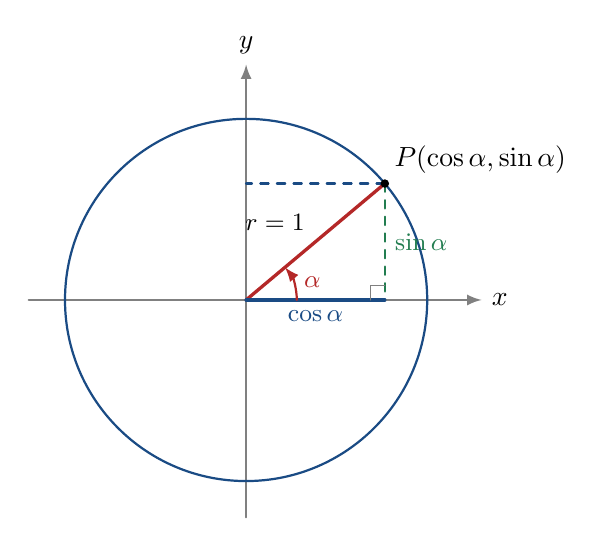
\begin{tikzpicture}[scale=2.3, cap=round, >=latex]
        % Koordináta-rendszer
        \draw[->, thick, gray] (-1.2,0) -- (1.3,0) node[right, black] {$x$};
        \draw[->, thick, gray] (0,-1.2) -- (0,1.3) node[above, black] {$y$};
        % Egységkör
        \draw[thick, matekKek] (0,0) circle (1cm);
        % Szög és pont
        \coordinate (O) at (0,0);
        \coordinate (P) at (40:1);
        \coordinate (Px) at ({cos(40)},0);
        \coordinate (Py) at (0,{sin(40)});
        
        % Vektor és háromszög
        \draw[very thick, matekPiros] (O) -- (P) node[midway, above left, black] {\small $r=1$};
        \draw[dashed, matekZold, thick] (P) -- (Px) node[midway, right] {\small $\sin\alpha$};
        \draw[dashed, matekKek, thick] (P) -- (Py);
        \draw[very thick, matekKek] (O) -- (Px) node[midway, below] {\small $\cos\alpha$};
        
        % Derékszög jele
        \draw[gray] (Px) ++(0,0.08) -- ++(-0.08,0) -- ++(0,-0.08);
        
        % Szög íve
        \draw[->, thick, matekPiros] (0.28,0) arc (0:40:0.28) node[midway, right] {\small $\alpha$};
        \filldraw[black] (P) circle (0.02) node[above right] {$P(\cos\alpha, \sin\alpha)$};
    \end{tikzpicture}
\end{minipage}

\vspace{3mm}

\section{Definíciós összefüggések és reciprok relációk}

A tangens és kotangens függvényeket a szinusz és koszinusz hányadosaként definiáljuk ott, ahol a nevező nem zéró:
\begin{multicols}{2}
\begin{itemize}[leftmargin=5mm]
    \item $\tan\alpha = \dfrac{\sin\alpha}{\cos\alpha} \quad \left(\alpha \neq \frac{\pi}{2} + k\pi, \; k \in \mathbb{Z}\right)$
    \item $\cot\alpha = \dfrac{\cos\alpha}{\sin\alpha} \quad (\alpha \neq k\pi, \; k \in \mathbb{Z})$
\end{itemize}
\end{multicols}

\noindent Ebből közvetlenül következik a tangens és kotangens szorzata:
\[
\tan\alpha \cdot \cot\alpha = 1 \implies \cot\alpha = \frac{1}{\tan\alpha}.
\]

\begin{kiemelt}[A tangens és a koszinusz kapcsolata]
Ha az alapegyenlet ($\sin^2\alpha + \cos^2\alpha = 1$) mindkét oldalát elosztjuk $\cos^2\alpha$-val ($\cos\alpha \neq 0$):
\[
\frac{\sin^2\alpha}{\cos^2\alpha} + \frac{\cos^2\alpha}{\cos^2\alpha} = \frac{1}{\cos^2\alpha} \iff 1 + \tan^2\alpha = \frac{1}{\cos^2\alpha}.
\]
Ez a formula rendkívül hasznos egyenletek megoldásakor, mert kapcsolatot teremt $\tan\alpha$ és $\cos\alpha$ között.
\end{kiemelt}

\vspace{2mm}

\section{Szimmetriák és redukciós formulák}

A trigonometrikus függvények páros, illetve páratlan tulajdonságai geometriailag azonnal leolvashatók az egységkörről:
\begin{center}
\renewcommand{\arraystretch}{1.3}
\begin{tabular}{|c|c|c|}
    \hline
    \textbf{Negatív szögek (Paritás)} & \textbf{Pótszögek összefüggései} & \textbf{Kiegészítő szögek} \\
    \hline
    $\cos(-\alpha) = \cos\alpha$ \text{(páros)} & $\sin\left(\frac{\pi}{2} - \alpha\right) = \cos\alpha$ & $\sin(\pi - \alpha) = \sin\alpha$ \\
    $\sin(-\alpha) = -\sin\alpha$ \text{(páratlan)} & $\cos\left(\frac{\pi}{2} - \alpha\right) = \sin\alpha$ & $\cos(\pi - \alpha) = -\cos\alpha$ \\
    $\tan(-\alpha) = -\tan\alpha$ \text{(páratlan)} & $\tan\left(\frac{\pi}{2} - \alpha\right) = \cot\alpha$ & $\tan(\pi - \alpha) = -\tan\alpha$ \\
    \hline
\end{tabular}
\end{center}

\newpage

\section{Addíciós tételek}

Az addíciós tételek segítségével két szög összegének vagy különbségének szinuszát és koszinuszát vezethetjük vissza az eredeti szögek függvényeire.

\begin{kiemelt}[Összeg és különbség trigonometrikus függvényei]
Tetszőleges $\alpha, \beta \in \mathbb{R}$ esetén érvényesek a következő azonosságok:
\begin{align}
    \sin(\alpha + \beta) &= \sin\alpha\cos\beta + \cos\alpha\sin\beta \\
    \sin(\alpha - \beta) &= \sin\alpha\cos\beta - \cos\alpha\sin\beta \\
    \cos(\alpha + \beta) &= \cos\alpha\cos\beta - \sin\alpha\sin\beta \\
    \cos(\alpha - \beta) &= \cos\alpha\cos\beta + \sin\alpha\sin\beta
\end{align}
Tangens esetén (amennyiben a nevezők nem zérók):
\[
\tan(\alpha \pm \beta) = \frac{\tan\alpha \pm \tan\beta}{1 \mp \tan\alpha\tan\beta}
\]
\end{kiemelt}

\begin{megjegyzes}
Figyeljük meg az előjeleket! A koszinusz esetében az összeghez kivonás, a különbséghez pedig összeadás tartozik: $\cos(\alpha \pm \beta) = \cos\alpha\cos\beta \mp \sin\alpha\sin\beta$.
\end{megjegyzes}

\section{Kétszeres szögek és linearizáló formulák}

Ha az addíciós tételekben a két szöget egyenlőnek választjuk ($\beta = \alpha$), megkapjuk a kétszeres szögek azonosságait:

\begin{multicols}{2}
    \begin{kiemelt}[Kétszeres szögek]
    \begin{align*}
        \sin(2\alpha) &= 2\sin\alpha\cos\alpha \\[2mm]
        \cos(2\alpha) &= \cos^2\alpha - \sin^2\alpha \\
                      &= 2\cos^2\alpha - 1 \\
                      &= 1 - 2\sin^2\alpha \\[2mm]
        \tan(2\alpha) &= \frac{2\tan\alpha}{1 - \tan^2\alpha}
    \end{align*}
    \end{kiemelt}
    
    \columnbreak
    
    \begin{kiemelt}[Linearizáló formulák (félszögek)]
    A $\cos(2\alpha)$ formuláinak átrendezéséből:
    \begin{align*}
        \sin^2\alpha &= \frac{1 - \cos(2\alpha)}{2} \\[3mm]
        \cos^2\alpha &= \frac{1 + \cos(2\alpha)}{2}
    \end{align*}
    Ezek a formulák csökkentik a hatványkitevőt, ami egyenletmegoldásban és integrálszámításban is kulcsfontosságú.
    \end{kiemelt}
\end{multicols}

\vspace{1mm}

\section{Kidolgozott mintapéldák}

\begin{pelda}[$\cos(75^\circ)$ pontos értékének kiszámítása]
\textbf{Feladat:} Határozzuk meg $\cos(75^\circ)$ pontos értékét négyzetgyökök segítségével!

\textbf{Megoldás:}\\
Bontsuk fel a $75^\circ$-os szöget olyan nevezetes szögek összegére, amelyeknek ismerjük az értékeit:
$75^\circ = 45^\circ + 30^\circ$.

Alkalmazzuk a koszinusz addíciós tételét:
\[
\cos(75^\circ) = \cos(45^\circ + 30^\circ) = \cos(45^\circ)\cos(30^\circ) - \sin(45^\circ)\sin(30^\circ)
\]
Helyettesítsük be a nevezetes értékeket:
\[
\cos(45^\circ) = \frac{\sqrt{2}}{2}, \quad \cos(30^\circ) = \frac{\sqrt{3}}{2}, \quad \sin(45^\circ) = \frac{\sqrt{2}}{2}, \quad \sin(30^\circ) = \frac{1}{2}
\]
Végezzük el a szorzást és a kivonást:
\[
\cos(75^\circ) = \left(\frac{\sqrt{2}}{2} \cdot \frac{\sqrt{3}}{2}\right) - \left(\frac{\sqrt{2}}{2} \cdot \frac{1}{2}\right) = \frac{\sqrt{6}}{4} - \frac{\sqrt{2}}{4} = \mathbf{\frac{\sqrt{6} - \sqrt{2}}{4}}.
\]
\end{pelda}

\begin{pelda}[Azonosság bizonyítása]
\textbf{Feladat:} Igazoljuk a következő azonosságot minden olyan $x$-re, ahol a kifejezések értelmezve vannak:
\[
\frac{\sin(2x)}{1 + \cos(2x)} = \tan x
\]

\textbf{Megoldás:}\\
Induljunk ki a bal oldalból, és használjuk a kétszeres szögekre vonatkozó formulákat:
\[
\text{Bal oldal (B)} = \frac{\sin(2x)}{1 + \cos(2x)}
\]
Tudjuk, hogy $\sin(2x) = 2\sin x \cos x$, valamint válasszuk a $\cos(2x) = 2\cos^2 x - 1$ alakot, hogy az $1$-es kieshessen:
\[
\text{B} = \frac{2\sin x \cos x}{1 + (2\cos^2 x - 1)} = \frac{2\sin x \cos x}{2\cos^2 x}
\]
Egyszerűsítsünk $2$-vel és $\cos x$-szel (mivel $\cos x \neq 0$):
\[
\text{B} = \frac{\sin x}{\cos x} = \tan x = \text{Jobb oldal (J)}.
\]
Ezzel az azonosságot bebizonyítottuk.
\end{pelda}

\begin{pelda}[Értékmeghatározás szögfüggvények kapcsolatával]
\textbf{Feladat:} Tudjuk, hogy $\sin\alpha = \frac{3}{5}$, és $\alpha$ a második síknegyedbe esik ($\frac{\pi}{2} < \alpha < \pi$). Számítsuk ki $\cos\alpha$ és $\sin(2\alpha)$ pontos értékét!

\textbf{Megoldás:}\\
1. A trigonometrikus alapegyenlet szerint: $\cos^2\alpha = 1 - \sin^2\alpha = 1 - \left(\frac{3}{5}\right)^2 = 1 - \frac{9}{25} = \frac{16}{25}$.\\
Mivel a második síknegyedben a koszinusz negatív, ezért:
\[
\mathbf{\cos\alpha = -\sqrt{\frac{16}{25}} = -\frac{4}{5}}.
\]
2. A kétszeres szög szinuszára vonatkozó összefüggés alapján:
\[
\mathbf{\sin(2\alpha)} = 2\sin\alpha\cos\alpha = 2 \cdot \left(\frac{3}{5}\right) \cdot \left(-\frac{4}{5}\right) = \mathbf{-\frac{24}{25}}.
\]
\end{pelda}

\vspace{1mm}

\section{Gyakorló feladatok}

\begin{enumerate}[itemsep=2mm]
    \item Számítsd ki $\sin(15^\circ)$ pontos értékét a $\sin(45^\circ - 30^\circ)$ felbontás segítségével!
    \item Igazold a következő azonosságot: $\dfrac{1 - \cos(2x)}{\sin(2x)} = \tan x$.
    \item Határozd meg $\cos(2\alpha)$ értékét, ha $\cos\alpha = -\dfrac{5}{13}$ és $\pi < \alpha < \dfrac{3\pi}{2}$!
\end{enumerate}

\end{document}